% draft会跳过文档中的所有图片。正式导出时需要删掉draft参数。
\documentclass[12pt, a4paper, oneside]{ctexart}

\usepackage{amsmath}
\usepackage{amssymb}
\usepackage{bm}
\usepackage{graphicx}
\usepackage{mathrsfs}
\usepackage{geometry}
\usepackage{framed}
\usepackage{color}
\usepackage{caption}
\usepackage{listings}
\usepackage{fancyhdr}
\usepackage{booktabs}
\usepackage{makecell}
\usepackage{indentfirst}
\usepackage{authblk}
\usepackage{multicol}
% \usepackage{draftwatermark}       % 需要应用水印时取消注释
\usepackage{enumitem}
\usepackage[hidelinks]{hyperref}
\usepackage{tikz}
\usepackage{ulem}
\usetikzlibrary{positioning, shapes.geometric}

% 分栏线宽
\columnseprule=0.4pt

% 定制第二级无序列表的点样式
\setlist[itemize,2]{label=$\diamond$}

\pagestyle{fancy}

\fancyhf{}      % 清空页眉页脚设置
\fancyhead[L] {
    % 工大计算机系logo
    
\includegraphics[height=7mm]{./images/logo1.jpg}
}
\fancyhead[C]{《计算机组成原理》复习}
\fancyhead[R]{\leftmark}    % 右侧页眉:当前章标题

% 页脚居中放置页码
\fancyfoot[C]{\thepage}

% 设置章节标题自动编号的格式
\ctexset{
  section/number=\chinese{section},
%   subsection/name={,},
%   subsection/number=\chinese{subsection}
}

% 行距。ctexart默认值为1.3
\linespread{1.2}

\lstset{
  language=pascal,
  basicstyle=\ttfamily,
  frame=single,
  numbers=left
}

% \SetWatermarkText{Eslzzyl整理}            % 设置水印内容
% \SetWatermarkLightness{0.9}             % 设置水印透明度 0-1
% \SetWatermarkScale{0.8}                   % 设置水印大小 0-1

\renewcommand{\headrulewidth}{1pt}  %页眉线宽,设为0可以去页眉线
\renewcommand{\footrulewidth}{1pt}  %脚注线的宽度

\definecolor{shadecolor}{RGB}{241, 241, 255}

\title{
    
\includegraphics[width=0.3\textwidth]{images/hfut-badge.pdf}
    
    \vspace{20pt}
    《计算机组成原理》总复习
}
\author{Eslzzyl}
\date{\today}

\newcounter{problemname}
\newenvironment{problem}{\begin{shaded}\stepcounter{problemname}\par\noindent\textbf{例题\arabic{problemname}. }}{\end{shaded}\par}
\newenvironment{solution}{\begin{shaded}\par\noindent\textbf{解答:}}{\end{shaded}\par}
% \newenvironment{solution}{\par\noindent\textbf{答案. }}{\par}
% \newenvironment{note}{\par\noindent\textbf{例题\arabic{problemname}的注记. }}{\\\par}
\newenvironment{note}{\par\noindent\textbf{注记. }}{\par}

\begin{document}

\maketitle
\newpage
\tableofcontents
\vspace{20pt}
% 如果在目录处有备注,可以写在这里。

\newpage

\section{计算机系统概述}

\subsection{计算机发展历程}

本节已从新大纲中删除,故略。

\subsection{计算机系统层次结构}

\subsubsection{计算机系统的组成}

计算机系统=硬件系统+软件系统

\subsubsection{计算机硬件}

\begin{enumerate}
  \item {\kaishu 冯·诺伊曼机基本思想}
  
  冯·诺依曼机有如下特点:
  \begin{itemize}
    \item 采用“存储程序”的工作方式,即:将事先编制好的程序和原始数据送入主存后才能执行,一旦程序被启动执行,就无需操作人员的干预,计算机会自动逐条执行指令,直至程序执行结束。
    \item 计算机硬件系统由5大部件组成:
    \begin{itemize}
      \item 运算器
      \item 存储器
      \item 控制器
      \item 输入设备
      \item 输出设备
    \end{itemize}
    \item 指令和数据以同等地位存储在存储器中,形式上没有区别,但计算机应当能够区分它们。
    \item 指令和数据均用二进制代码表示。指令由操作码和地址码组成。
  \end{itemize}
  \item {\kaishu 计算机的功能部件}
  \begin{enumerate}
    \item {\kaishu 输入设备}。如键盘、鼠标、扫描仪、摄像机等。
    \item {\kaishu 输出设备}。如显示器、打印机等。
    \item {\kaishu 存储器}
    
    又分主存(内存)和辅存(外存)。CPU可以直接访问主存,但不能直接访问辅存。
    
    主存的工作方式是按存储单元的地址进行存取,即\textbf{按地址存取方式}。

    MAR(存储器地址寄存器)、MDR(存储器数据寄存器)二者虽然属于存储器的一部分,但实际上是集成在CPU中的。
    \item {\kaishu 运算器}
    
    核心是ALU。此外还包含若干通用寄存器,如:
    \begin{itemize}
      \item 累加器 ACC
      \item 乘商寄存器 MQ
      \item 操作数寄存器 X
      \item 变址寄存器 IX
      \item 基址寄存器 BR
      
      前三个是必须的。
    \end{itemize}
    运算器还包含程序状态寄存器(PSW),又称标志寄存器。
    \item {\kaishu 控制器}
    
    包含如下组件:
    \begin{itemize}
      \item 程序计数器 PC
      \item 指令寄存器 IR
      \item 控制单元 CU
    \end{itemize}
  \end{enumerate}
\end{enumerate}

\subsubsection{计算机软件}

\begin{enumerate}
  \item {\kaishu 系统软件和应用软件}
  
  系统软件:操作系统、数据库\textbf{管理系统}、语言处理程序、分布式软件系统、网络软件系统、标准库程序、服务性程序等。
  应用软件:各种科学计算类程序、工程设计类程序、数据统计与处理程序等。
  \item {\kaishu 三个级别的语言}
  \begin{enumerate}
    \item 机器语言。
    \item 汇编语言。
    \item 高级语言。
  \end{enumerate}
  将高级语言/汇编语言程序转换为机器语言程序的软件系统称为翻译程序,具体有以下三类:
  \begin{enumerate}
    \item 汇编程序(汇编器)
    \item 解释程序(解释器)
    \item 编译程序(编译器)
  \end{enumerate}
  \item {\kaishu 软件和硬件的逻辑功能等价性}

  对某一功能来说,既可以由硬件实现,又可以由软件实现,对于用户来说,它们在功能上是等价的。

  硬件实现的性能往往优于软件实现。
\end{enumerate}

\subsubsection{计算机系统的层次结构}

\begin{figure}[h]
  \centering
  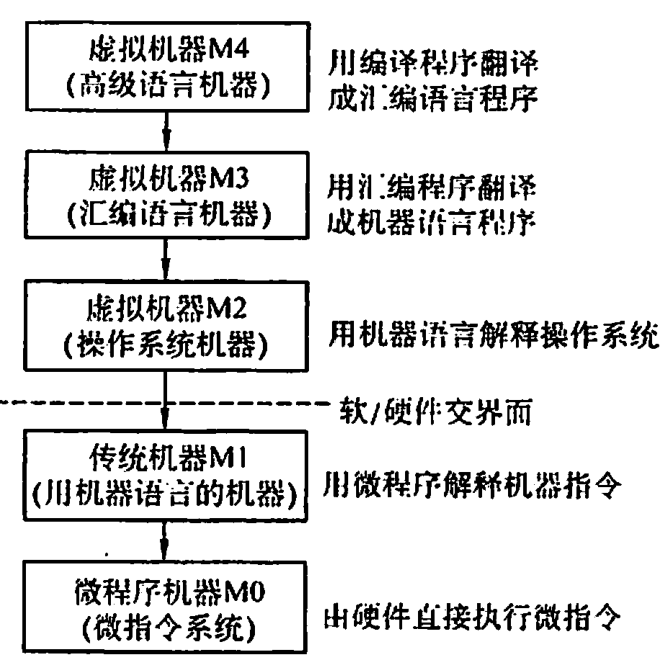
\includegraphics[width=0.4\textwidth]{./images/computer_system_layer.png}
  \caption{计算机系统的多级层次结构}
  \label{computer_system_layer}
\end{figure}

如图\ref{computer_system_layer}所示:
\begin{itemize}
  \item 第一级是微程序机器层,是实在的硬件层。
  \item 第二级是传统机器语言层,也是实在的硬件层。
  \item 第三级是操作系统层,这一层也成为混合层。
  \item 第四级是汇编语言层。
  \item 第五级是高级语言层。
\end{itemize}

软件和硬件的交界面就是ISA。

\subsubsection{计算机系统的工作原理}

\begin{enumerate}
  \item {\kaishu 从源程序到可执行文件}
  
  gcc编译流程:预处理-编译-汇编-链接
  \item {\kaishu 指令执行过程的描述}
  \begin{enumerate}
    \item 取指令:PC$\to$MAR$\to$M$\to$MDR$\to$IR
    \item 分析指令:OP(IR)$\to$CU
    \item 执行指令:Ad(IR)$\to$MAR$\to$M$\to$MDR$\to$ACC
  \end{enumerate}
  表示数据通路时括号可以省略,但运算时括号不能省略。如果题目中的括号没有省略,答题时也最好不要省略。
\end{enumerate}

\begin{problem}
  冯·诺依曼机的基本工作方式是 \uline{控制流驱动方式}。
\end{problem}

\begin{problem}
  下列(\ \ )不属于系统软件。
  \begin{enumerate}
    \item [A. ] 数据库系统
    \item [B. ] 操作系统
    \item [C. ] 编译程序
    \item [D. ] 以上三种都属于系统程序
  \end{enumerate}
\end{problem}

\begin{solution}
  A.本题易误选D。注意数据库系统=数据库+数据库管理系统+应用系统+数据库管理员,其中仅数据库管理系统是系统程序。
\end{solution}

\begin{problem}
  相联存储器 \uline{既可按地址寻址又可按内容寻址}。
\end{problem}

\begin{problem}
  【2009统考】冯·诺依曼计算机中指令和数据均以二进制形式存放在存储器中,CPU区分它们的依据是(\ \ )
  \begin{enumerate}
    \item [A. ] 指令操作码的译码结果
    \item [B. ] 指令和数据的寻址方式
    \item [C. ] 指令周期的不同阶段
    \item [D. ] 指令和数据所在的存储单元
  \end{enumerate}
\end{problem}

\begin{solution}
  C。通常取指阶段取出的是指令,执行阶段取出的是数据。
\end{solution}

\subsection{计算机的性能指标}

\subsubsection{计算机的主要性能指标}

\begin{enumerate}
  \item {\kaishu 字长},指计算机进行一次整数运算所能处理的二进制数据的位数。
  \item {\kaishu 数据通路带宽}
  \item {\kaishu 主存容量}。MAR的位数反映了存储单元的个数,MDR的位数反映了存储单元的字长。
  \item {\kaishu 运算速度}
  \begin{enumerate}
    \item 吞吐量,主要取决于主存的存储周期。
    \item 响应时间,通常包括CPU时间和等待时间。
    \item CPU时钟周期,是主频的倒数,是CPU中最小的时间单位。
    \item 主频。
    \item CPI:执行一条指令所需要的时钟周期数。一般是一个平均值。
    \item CPU执行时间
    \item MIPS:百万条指令每秒
    \item 浮点操作次数每秒系列单位:MFLOPS、GFLOPS、TFLOPS、PFLOPS、EFLOPS、ZFLOPS、EFLOPS
  \end{enumerate}
  注意:在描述存储容量、文件大小等时,K、M、G、T通常用2的幂次表示,而描述速率、频率等时,通常用10的幂次表示。
\end{enumerate}

\begin{problem}
  从用户观点看,评价计算机系统性能的综合参数是(\ \ )
  \begin{enumerate}
    \item [A. ] 指令系统
    \item [B. ] 吞吐率
    \item [C. ] 主存容量
    \item [D. ] 主频
  \end{enumerate}
\end{problem}

\begin{solution}
  B
\end{solution}

\section{数据的表示和运算}

\subsection{数制与编码}

\subsubsection{进位计数制及其相互转换}

计算机系统中所有信息都用二进制编码的原因:
\begin{itemize}
  \item 使用有两个稳定状态的物理器件就可以表示二进制数的每一位,成本低廉。
  \item 二进制的“0”和“1”恰好与逻辑值“真”和“假”相对应。
  \item 二进制的编码和运算规则都比较简单。
\end{itemize}

\begin{enumerate}
  \item {\kaishu 进位计数法}
  
  一个$r$进制数($K_n K_{n-1}\cdots K_0 K_{-1}\cdots K_{-m}$)的数值可表示为
  \begin{equation*}
    K_n r^n+K_{n-1}r^{n-1}+\cdots+K_0 r^0+K_{-1}r^{-1}+\cdots+K_{-m}r^{-m}=\sum_{i=n}^{-m}K_i r^i
  \end{equation*}
  式中,$r$是基数;$r^i$是第$i$位的位权(整数位最低规定为第0位);$K_i$的取值可以是$0,1,\cdots,r-1$共$r$个数码中的任意一个。
  \item {\kaishu 不同进制数之间的相互转换}
  \begin{enumerate}
    \item 二进制转八进制和十六进制
    
    二进制混合数(整数+小数)的整数部分,高位补0至对齐(转八进制则对齐到3位的整数倍,转十六进制则对齐到4位的整数倍);小数部分,低位补0至对齐,然后直接转换。

    八、十六进制互转时,可借助二进制作为中介。
    \item 任意进制数转为十进制数:各位数码和权值相乘然后加起来
    \item 十进制数转为任意进制数
    
    将十进制混合数拆成整数部分和小数部分,整数部分除基取余,小数部分乘基取整,最后再拼接起来。

    乘基取整:小数部分乘基取整,最先取得的整数为数的最高位,最后取得的整数为数的最低位,乘基为1.0或满足精度要求时结束。

    每个二进制小数都可以用十进制小数精确表示,但反之则不一定。
  \end{enumerate}
\end{enumerate}

\subsubsection{BCD码}

本节已从新大纲中删除,故略。

\subsubsection{定点数的编码表示}

\begin{enumerate}
  \item 机器数的定点表示
  \item 原码、反码、补码、移码
  \begin{enumerate}
    \item 原码表示法
    
    \begin{itemize}
      \item 若字长为$n+1$,则原码\textbf{小数}的表示范围为$-(1-2^{-n})\leq x\leq 1-2^{-n}$(关于原点对称)
      \item 若字长为$n+1$,则原码\textbf{整数}的表示范围为$-(2^{n}-1)\leq x\leq 2^{n}-1$(关于原点对称)
    \end{itemize}

    真值0的原码表示有两种,即+0和-0。
    \item 补码表示法
    
    小数补码比原码多表示一个-1,整数补码比原码多表示一个-2。

    变形补码:又称模4补码,双符号位的补码小数,符号位00表示正,11表示负。模4补码的符号位的存储仅仅需要\textbf{一位}而不是两位,因为任何一个正确的模4补码,符号位的两位都是相同的,如果不同表示发生了溢出。

    补码真值互转:整数直接按原码转换,负数则各位取反加1。

    另一种方法:从后往前找到第一个1,该1不变,前面所有位(含符号位)取反,符号去掉即可。
    \item 反码表示法
    \item 移码表示法
    
    移码就是在真值上加一个偏置值:
    \begin{equation*}
      [x]_{\text{移}}=2^n+x\ (-2^n\leq x< 2^n\text{,其中机器字长为}n+1)
    \end{equation*}
    移码有如下特点:
    \begin{itemize}
      \item 0的表示是唯一的。
      \item 同一个真值的补码和移码只差一个符号位。补码符号位取反,数值部分不变即得移码,反之亦然。
      \item 移码保持了数据的原有大小顺序,移码大真值就大,移码小真值就小。
    \end{itemize}
  \end{enumerate}
\end{enumerate}

\subsubsection{整数的表示}

\begin{enumerate}
  \item {\kaishu 无符号整数的表示}
  \item {\kaishu 带符号整数的表示}
\end{enumerate}

\begin{problem}
  对于相同位数(设为$N$位,不考虑符号位)的二进制补码小数和十进制小数,比值$\frac{\text{二进制小数能表示的数的个数}}{\text{十进制小数能表示的数的个数}}$为 \uline{$(0.2)^N$}
\end{problem}

\begin{solution}
  $N$位二进制小数可以表示的数的个数为$1+2^0+2^1+\cdots+2^{N-1}=2^N$,而十进制小数能表示的数的个数为$10^N$,二者的商为$(0.2)^N$。这也是计算机的运算中会出现误差的原因,它表明仅有$(0.2)^N$的概率的十进制数可以精确地用二进制表示。
\end{solution}

\subsection{运算方法和运算电路}

\subsubsection{基本运算部件}

408很少涉及本节内容。

加法器是ALU的核心部件。

\begin{enumerate}
  \item {\kaishu 一位全加器}
  \item {\kaishu 串行进位加法器}
  
  串行进位加法器的最长运算时间主要是由进位信号的传递时间决定的,加法器本身的求和时间只是次要因素。
  \item {\kaishu 并行进位加法器}
  \item {\kaishu 带标志加法器}
  \item {\kaishu 算数逻辑单元(ALU)}
\end{enumerate}

\subsubsection{定点数的移位运算}

\begin{enumerate}
  \item {\kaishu 算术移位}
  
  算术移位的对象是\textbf{有符号数}。

  算术移位不管怎么移,符号位永远是不变的,也即移位只作用于数值位。

  \begin{itemize}
    \item 正数无论码制,左右移都一律补0。
    \item 负数稍复杂:
    \begin{itemize}
      \item 原码:一律补0
      \item 反码:一律补1
      \item 补码:左移补0,右移补1
    \end{itemize}
  \end{itemize}

  \begin{table}[!ht]
    \centering
    \caption{不同机器数算术移位后的空位添补规则}
    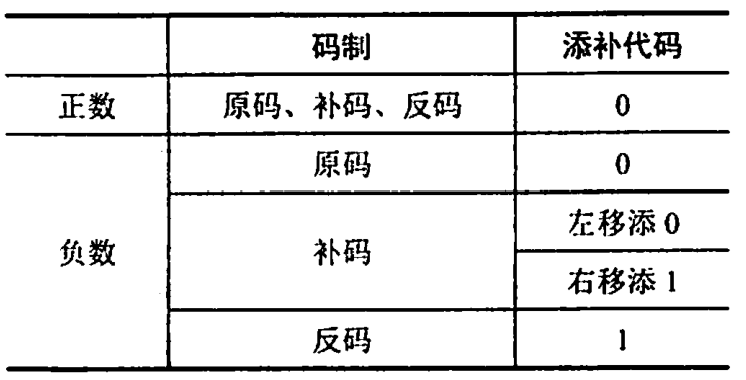
\includegraphics[width=0.6\textwidth]{./images/shift_rule.png}
  \end{table}
  \item {\kaishu 逻辑移位}
  
  逻辑移位将移位对象视为\textbf{无符号数}。无论码制、左右移,一律补0。
  \item {\kaishu 循环移位}
  
  又分带进位标志CF的循环移位和不带进位标志的循环移位。

  带CF的循环移位是将移出的位送入标志位CF,并将CF的值送入腾出的位。

  即使是不带CF的循环移位,实际上CF的值也是会变的,但CF只是单纯输入,不再输出。输入的值是移出的位。

  循环移位操作常用于交换寄存器的高低字节。
\end{enumerate}

\subsubsection{定点数的加减运算}

\begin{enumerate}
  \item {\kaishu 补码的加减法运算}
  \item {\kaishu 补码加减运算电路}
  
  这里有一个各标志位的含义,可能有用。待补。
  \item {\kaishu 溢出判别方法}
  
  仅当两个符号相同的数相加或者两个符号相异的数相减才有可能产生溢出。判断溢出的方法有三种:
  \begin{itemize}
    \item 采用一位符号位:无论加减,只要参加操作的两个数符号相同,结果又与源操作数符号不同,就表示溢出。
    \item 采用双符号位:运算结果的两个符号位相同,表示未溢出;若不同则表示溢出。
    \begin{itemize}
      \item 00:表示结果为正,无溢出。
      \item 01:表示结果正溢出。
      \item 10:表示结果负溢出。
    \end{itemize}
    \item 采用一位符号位根据数据位的进位情况判断溢出
    
    当最高符号位的进位和数值位的进位不同时,说明发生溢出。
  \end{itemize}
\end{enumerate}

\subsubsection{定点数的乘除运算}

待补

\subsubsection{C语言中的整数类型及类型转换}

本节为408常考内容。

当大字长变量向小字长变量强制类型转换时,多余的高位直接截掉,低位直接赋值,而不是进行类似循环溢出的操作。

短字长向长字长转换时,不仅要使相应的位值相等,还要对高位进行扩展:
\begin{itemize}
  \item 如果原数字是无符号整数,则进行零扩展
  \item 如果原数字带符号,则进行符号扩展。
\end{itemize}

char类型为8位无符号整数,转为int时高位补0即可。

\subsubsection{数据的存储和排列}

\begin{enumerate}
  \item {\kaishu 数据的“大端方式”和“小端方式”存储}
  \begin{itemize}
    \item 大端:低字节放高地址
    \item 小端:低字节放低地址
  \end{itemize}
  \item {\kaishu 数据按“边界对齐”方式存储}
  
  \textbf{注意}:题目涉及\textbf{结构体}的,一定要留意对齐方式(一般都是边界对齐的)!
\end{enumerate}

\subsection{浮点数的表示与运算}

\subsubsection{浮点数的表示}

\begin{enumerate}
  \item {\kaishu 浮点数的表示格式}
  
  通常,浮点数可表示为
  \begin{equation*}
    N=(-1)^S\times M\times R^E
  \end{equation*}
  其中:
  \begin{itemize}
    \item $S$决定浮点数的符号,可取0或1。
    \item $M$是尾数,是一个二进制定点小数,通常用原码表示。
    \item $E$是阶码,是一个二进制定点整数,通常用移码表示。
    \item $R$是隐含的基数,可取2、4、16等。
  \end{itemize}
  \item {\kaishu 浮点数的表示范围}
  
  \begin{itemize}
    \item 数据产生上溢(正上溢、负上溢)时,计算机必须停机处理溢出。
    \item 数据产生下溢(正下溢、负下溢)时,计算机将其当作机器零处理。
  \end{itemize}
  \item {\kaishu 浮点数的规格化}
  
  \begin{itemize}
    \item 左规:尾数的最高位不是有效位,即尾数为$0.0\cdots$时,进行左规,尾数每左移一次,阶码减一(仅基数为2时)。
    \item 右规:尾数的有效位进到小数点前面时,进行右规,尾数右移一位,阶码加一(仅基数为2时)。
  \end{itemize}

  基数不同,浮点数的规格化形式也不同。基数为2时,原码规格化数的尾数最高位一定是1;基数为4时,原码规格化形式的尾数最高两位不全为0。
  \item {\kaishu IEEE 754标准}
  
  IEEE 754规定:浮点数的基数隐含为2,尾数采用隐藏位策略的原码表示,阶码用移码表示。
  \begin{table}
    \centering
    \caption{IEEE 754浮点数的格式}
    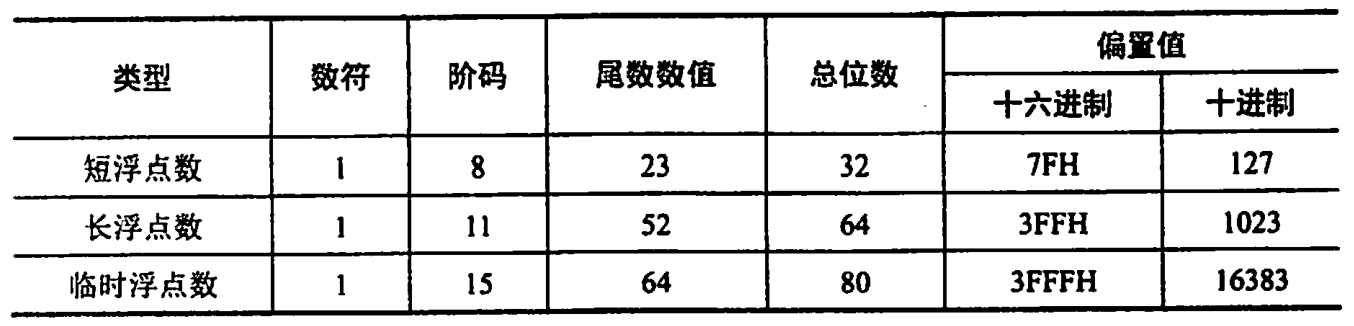
\includegraphics[width=0.7\textwidth]{./images/ieee754.png}
  \end{table}
  对于短浮点数,偏置值为127;对于长浮点数,偏置值为1023。存储阶码之前,要先把真值加上偏置值;反之在解析真值时,需要将阶码减去偏置值。

  规格化的二进制浮点数,数值最高位总是1,因此此位省略,尾数实际上能多表示一位有效位。
  \item {\kaishu 定点、浮点表示的区别}
\end{enumerate}

\subsubsection{浮点数的加减运算}

分为以下几步:
\begin{enumerate}
  \item {\kaishu 对阶}
  
  原则是小阶向大阶对齐,即将阶码数小的浮点数的阶码逐位增加1,同时尾数逐位右移,直到两个数阶码相等为止。
  \item {\kaishu 尾数求和}
  \item {\kaishu 规格化}
  
  尾数求和的结果不一定是规格化的,因此需要规格化。
  \item {\kaishu 舍入}
  
  为保证精度,一般将右移移出的位保留下来,在最后得出结果时舍入成IEEE 754格式。
  \begin{itemize}
    \item 0舍1入法:类似四舍五入。若保留下来的最高位为1,则在尾数的末位加1,否则就舍去。
    \item 恒置1法:无脑将右移后的尾数末位置为1。
    \item 截断法:直接截断,最简单。
  \end{itemize}
  \item {\kaishu 溢出判断}
\end{enumerate}

\section{存储系统}

\subsection{存储器概述}

\subsubsection{存储器的分类}

\begin{enumerate}
  \item {\kaishu 按在计算机中的作用(层次)分类}
  \begin{itemize}
    \item 主存储器
    \item 辅助存储器
    \item 高速缓冲存储器(Cache)
  \end{itemize}
  \item {\kaishu 按存储介质分类}
  \begin{itemize}
    \item 磁表面存储器(磁盘、磁带)
    \item 磁芯存储器
    \item 半导体存储器
    \begin{itemize}
      \item MOS型存储器
      \item 双极型存储器
    \end{itemize}
    \item 光存储器(光盘)
  \end{itemize}
  \item {\kaishu 按存取方式分类}
  \begin{itemize}
    \item 随机存储器(RAM):又分静态RAM和动态RAM
    \item 只读存储器(ROM):可与RAM共同作为主存的一部分,统一构成主存的地址域。同样支持随机访问。
    \item 串行访问存储器。包括:
    \begin{itemize}
      \item 顺序存取存储器(如磁带)
      \item 直接存取存储器(如磁盘、光盘)
    \end{itemize}
  \end{itemize}
  \item {\kaishu 按信息的可保存性分类}
  \begin{itemize}
    \item 易失性存储器,如RAM
    \item 非易失性存储器,如ROM、磁表面存储器和光存储器。
  \end{itemize}
\end{enumerate}

\subsubsection{存储器的性能指标}

三大性能指标:
\begin{enumerate}
  \item 存储容量。=存储字数$\times$字长
  \item 单位成本。
  \item 存储速度。
\end{enumerate}

与存储速度有关的几个概念:
\begin{itemize}
  \item 存取时间
\end{itemize}

\section{指令系统}

\section{中央处理器}

\section{总线}

\section{输入/输出系统}

\end{document}